\section{Performance}\label{sec:performance}
%\matthias{This is the working ProB code that we'll show as an example}
%In this section, the graph mining problem is slightly modified: we now restrict the search for a pattern to graphs that are a subgraph of a given \emph{template} graph.
%The declarative approach allows us to implement such a modification with only minimal effort.
%\VerbatimInput{original_prob_files/PositiveAndNegative.mch}

In Listing~\ref{lst:IDPPos}, we show part of the working model for the graph mining problem (for complete encodings, we refer to the appendix).
It shows the constraints necessary to enforce the positive homomorphic property.
As one would desire due to the similarity underlying the two homomorphic constraints, the theory expressing the negative homomorphic property is the same except for the threshold.
\todo{Michael, could you think of a snippet of code for ProB? Preferrably, we would also use as much of the same terminology as possible as in idp/asp.}

%\begin{lstlisting}[caption=IDP positive constraint, style=model, label=lst:IDPPos]
%vocabulary V{
%  type node isa nat
%  type graphid
%  type label
%
%  // Predicates determining the template graph.
%  template_edge(node, node) 
%  template_label(node):label
%
%  // Predicates describing the positive example graphs
%  example_edge(graphid, node, node)
%  label(graphid, node):label
%  threshold: int
%
%  // Predicates describing the pattern graph
%  inpattern(node) // True for the nodes which occur in the pattern
%  partial f(graphid, node):node // Represents the homomorphisms with the example graphs
%  homowith(graphid) // True for graphs for which f represents a correct homomorphism
%  path(node, node) // path(a,b): True if there exists a path from a to b in the pattern
%}
%
%theory Positive:V_Pos{
%   //The pattern is a connected subgraph of the template: From every node in the pattern, 
%   //there exists a path to every other node in the pattern.
%   !x,y[node] : x ~= y & inpattern(x) & inpattern(y) => path(x,y).
%   {
%      path(x,y) <- template_edge(x,y) & inpattern(x) & inpattern(y).
%      path(x,y) <- ?z[node] : path(x,z) & path(z,y).
%      path(x,y) <- path(y,x).
%   }
%
%   //existence of a homomorphic f from the pattern to example graph with graphid gid.
%   !gid[graphid] : !x[node]   : homowith(gid) & inpattern(x) <=> ? y[node] : y=f(gid,x).
%   !gid[graphid] : !x,y[node] : homowith(gid) & inpattern(x) & inpattern(y) & x~=y => f(gid, x) ~= f(gid,y).
%   !gid[graphid] : !x,y[node] : homowith(gid) & inpattern(x) & inpattern(y) & template_edge(x,y) => edge(gid, f(gid,x). f(gid,y)).
%   !gid[graphid] : !x[node] : homowith(gid) & inpattern(x) => template_label(x) = label(gid, f(gid,x)).
%
%   // At least N homomorphisms must be found
%   #{ gid [graphid] : homowith(graph) } >= threshold.
%}
%\end{lstlisting}
%
%
%\lstset{basicstyle=\footnotesize\ttfamily,breaklines=true}
%\begin{lstlisting}[caption=ASP positive matching, style=model]
%homowith(G) | not_homowith(G) :- positive(G).
%
%1 { f(G,X,V) : node(G,V) } 1 :- positive(G), inpattern(X).
%
%:- homo_with(G), f(G,X,V1), f(G,Y,V2), template_edge(X,Y), 
%not edge(G,V1,V2), inpattern(X), inpattern(Y).
%
%positive_count(N) :- N = #count{G:homowith(G)}.
%
%:- positive_count(N), N < 2.
%\end{lstlisting}
%
%\begin{lstlisting}[caption=ASP negative matching using saturation technique, label={lst:aspsaturation}, style=model, numbers=left]
%map(G,X,v1) | map(G,X,v2) | map(G,X,v3) | map(G,X,v4) :- invar(X), negative(G). @\label{lstline:probspec}@
%map(G,X,V) :- saturated(G), t_node(X), node(G,V).
%
%saturated(G) :- t_edge(X,Y), map(G,X,V1), map(G,Y,V2), not edge(G,V1,V2), negative(G), invar(X), invar(Y).
%saturated(G) :- map(G,X,V),  map(G,Y,V), X != Y, invar(X), invar(Y). // we cannot map two different template nodes to the same 
%
%neg_homowith(G) :- not saturated(G), negative(G).
%
%negative_count(N) :- N = #count{G:neg_homowith(G)}.
%:- negative_count(N), N > 1.
%
%\end{lstlisting}
%\todo{Sergey: Why is the canonicity template-based check so different from the negative maching specification. In the negative matchin, all that is added is the saturated predicate, is it not possible to add only that in the case of canonicity?}

%\begin{lstlisting}[caption=Canonicity template-based check, style=model]
%iso(X,x1) | iso(X,x2) | iso(X,x3) | iso(X,x4) :- invar(X).
%
%candidate_var(X) :- iso(_,X).
%
%%not iso!
%iso_saturated :- invar(X1), invar(X2), iso(X1,V1), iso(X2,V2),     t_edge(V1,V2), not t_edge(X1,X2). 
%iso_saturated :- invar(X1), invar(X2), iso(X1,V1), iso(X2,V2), not t_edge(V1,V2),     t_edge(X1,X2).
%
%iso(X,V) :- invar(X), t_node(V), iso_saturated.
%
%d1(X) :-     invar(X), not candidate_var(X). 
%d2(X) :- not invar(X),     candidate_var(X).
%
%not_equal :- d1(X). % check that in fact candidate is different from the pattern itself
%not_equal :- d2(X). % check that in fact candidate is different from the pattern itself
%
%iso_saturated :- not not_equal. % should not be completely equal
%
%min_d1(N) :- N = #min{ X: d1(X) }, not iso_saturated.
%min_d2(N) :- N = #min{ X: d2(X) }, not iso_saturated.
%
%iso_saturated :- min_d1(N1), min_d2(N2), N1 > N2.
%\end{lstlisting}
%
%\begin{lstlisting}[caption=Auxilary predicates -- probably should be moved to appendix, style=model]
%%selects subpattern
%
%t_path(X,Y) :- t_edge(X,Y), invar(X), invar(Y).
%t_path(X,Y) :- t_edge(X,Z), t_path(Z,Y), invar(X).
%
%:- invar(X), invar(Y), not t_path(X,Y).
%
%0 { invar(X) } 1 :- t_node(X).
%% auxilary constraints
%
%
%edge(G,Y,X) :- edge(G,X,Y).
%t_edge(Y,X) :- t_edge(X,Y).
%node(G,Y)   :- edge(G,Y,_).
%t_node(X)   :- t_edge(X,_).
%\end{lstlisting}

%\begin{lstlisting}[caption=Canonicity previous solution isomorphism check, style=model]
%iso(s1,X,x1) | iso(s1,X,x2) :- invar(X).
%iso(s2,X,x2) | iso(s2,X,x3) :- invar(X).
%
%candidate_var(G,X) :- iso(G,_,X).
%
%iso_saturated(G) :- invar(X1), invar(X2), iso(G,X1,V1), iso(G,X2,V2),     t_edge(V1,V2), not t_edge(X1,X2). 
%iso_saturated(G) :- invar(X1), invar(X2), iso(G,X1,V1), iso(G,X2,V2), not t_edge(V1,V2),     t_edge(X1,X2). 
%iso_saturatea(G) :- not equal(G), iso(G,_,_). 
%
%iso(G,X,V) :- invar(X), t_node(V), iso_saturated(G).
%
%:- not iso_saturated(G), iso(G,_,_).
%
%d1(G,X) :-     invar(X), not candidate_var(G,X), iso(G,_,_).
%d2(G,X) :- not invar(X),     candidate_var(G,X).
%
%not_equal(G) :- d1(G,X). % check that in fact candidate is different from the pattern itself
%not_equal(G) :- d2(G,X). % check that in fact candidate is different from the pattern itself
%
%equal(G) :- not not_equal(G), iso(G,_,_).
%
%\end{lstlisting}
We compared the performance of the different encoding techniques on the mutagenesis~\citep{?} dataset for graph mining.
First, we randomly picked a positive example to use as the template graph.
Next, we mined a random sample subset of the mutagenesis dataset for $n$ canonical patterns with thresholds $N_{+} = $ 5\% of the size of the positive example set, and $N_{-} =$ 5\% of the size of the negative example set.
During the mining process, we tracked the time it takes to mine the $i=1..n$'th pattern.
The results shown are the times needed to mine the $i$'th pattern, averaged over * repeats of the process above.

\begin{figure}
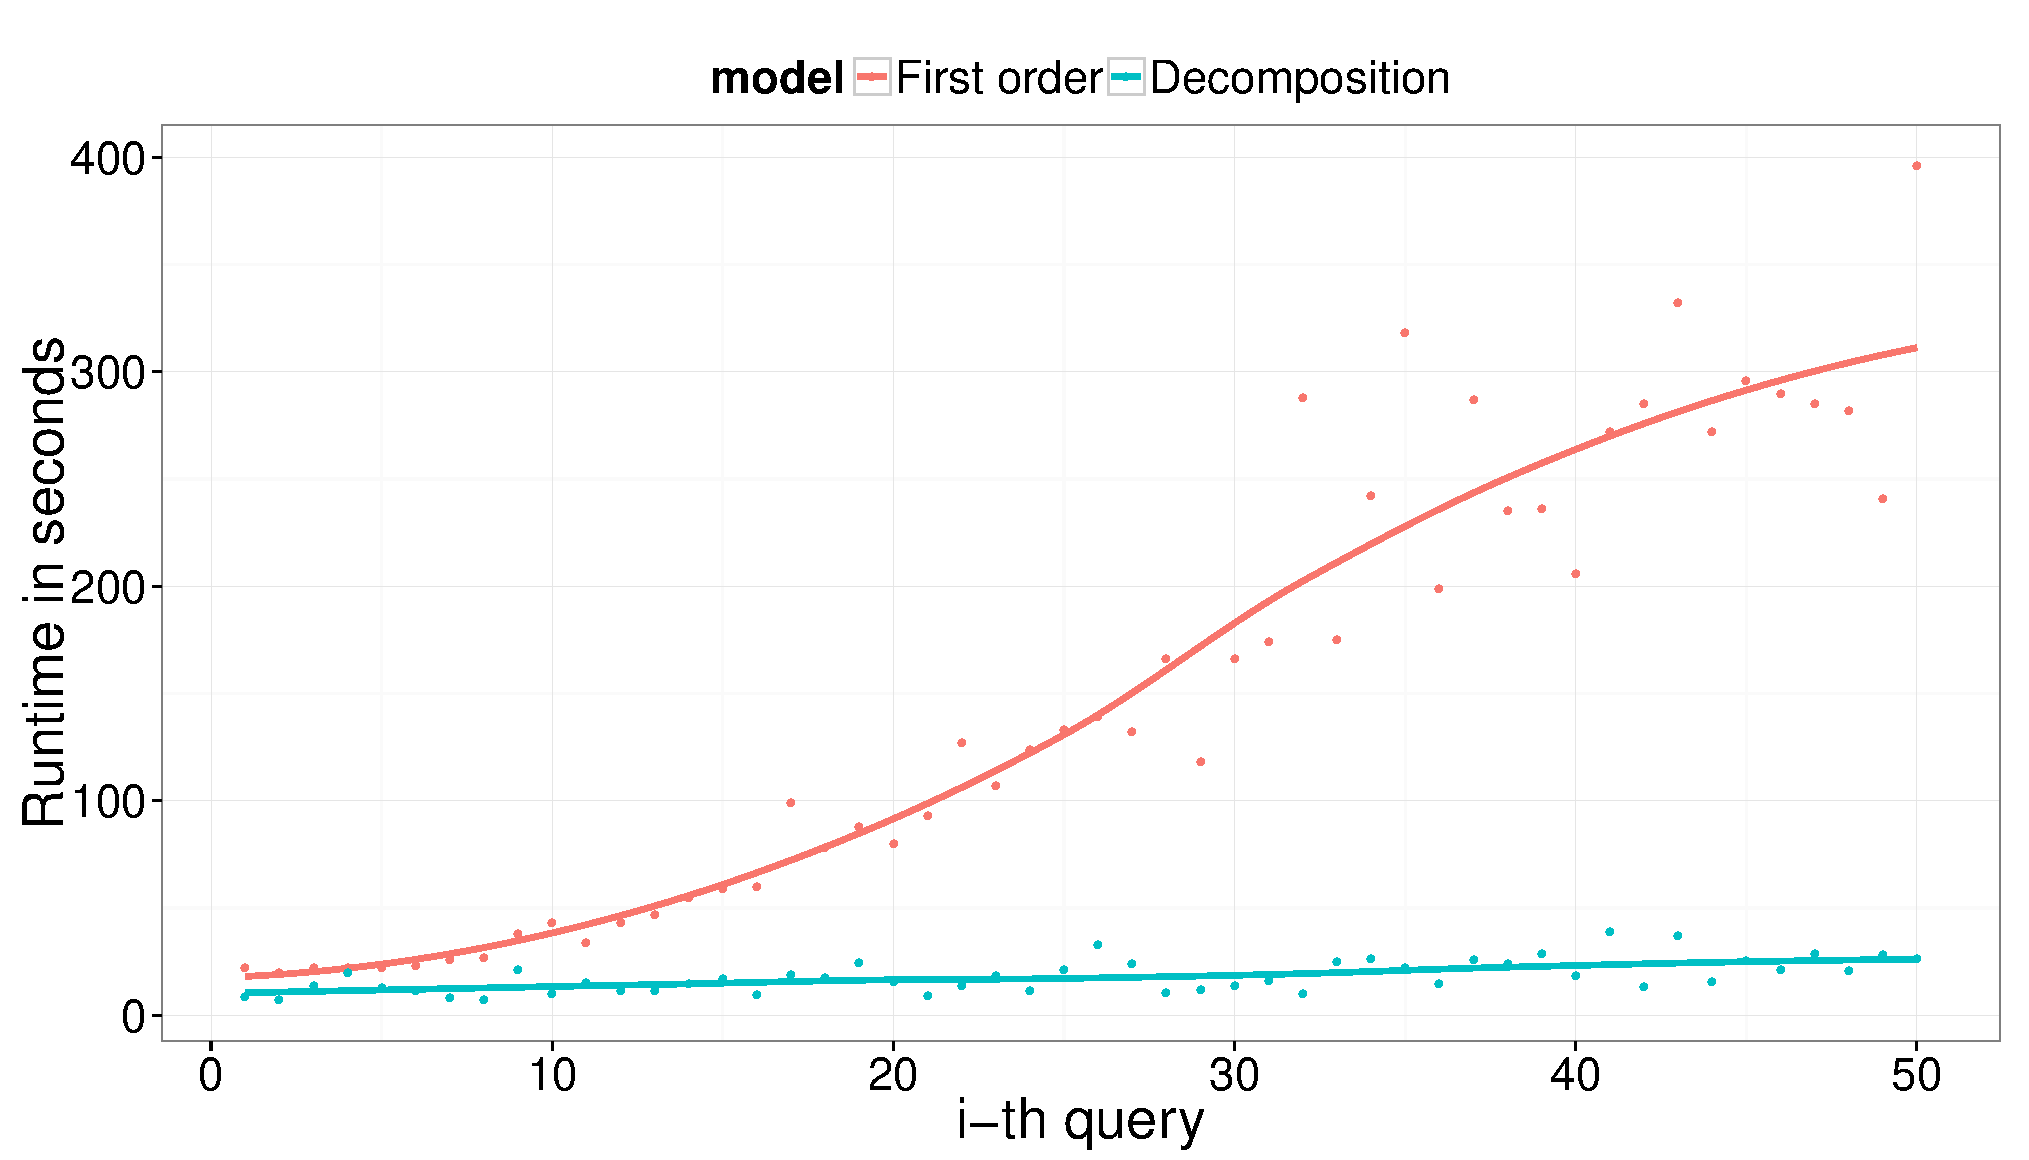
\includegraphics[scale=0.20]{extra/figure_comparison_yoshida.pdf}
\end{figure}
